\documentclass{article}
\usepackage{pgfplots}
\pgfplotsset{compat=1.17}


\begin{document}

% Figure # 1
\begin{figure}
    \centering
    
\begin{tikzpicture}
  \definecolor{navy}{RGB}{0, 0, 128}
  \definecolor{dimgray85}{RGB}{85, 85, 85}
  \definecolor{darkorange}{RGB}{255, 140, 0}
  \definecolor{lightgray}{RGB}{211, 211, 211}
  \definecolor{lightgray204}{RGB}{204, 204, 204}

  \begin{axis}[
    legend style={
      fill opacity=0.8,
      draw opacity=1,
      text opacity=1,
      at={(0.97,0.03)},
      anchor=south east,
      draw=lightgray204a
    },
    grid=major,
    tick pos=left,
    xmin=0, xmax=1,
    ymin=0, ymax=1,
    title={ROC Curve},
    tick align=outside,
    ylabel=\textcolor{dimgray85}{True Positive Rate},
    xlabel=\textcolor{dimgray85}{False Positive Rate},
    xtick={0, 0.2, 0.4, 0.6, 0.8, 1},
    ytick={0, 0.2, 0.4, 0.6, 0.8, 1},
  ]
    \addplot[thick, darkorange] coordinates {(0.0, 0.0)(0.01, 0.0)(0.01, 0.01)(0.03, 0.01)(0.03, 0.02)(0.04, 0.02)(0.04, 0.05)(0.07, 0.05)(0.07, 0.13)(0.08, 0.13)(0.08, 0.15)(0.08, 0.16)(0.1, 0.16)(0.1, 0.17)(0.11, 0.17)(0.11, 0.23)(0.15, 0.23)(0.15, 0.25)(0.16, 0.25)(0.16, 0.26)(0.17, 0.26)(0.17, 0.27)(0.22, 0.27)(0.22, 0.28)(0.22, 0.3)(0.25, 0.3)(0.25, 0.33)(0.25, 0.34)(0.28, 0.34)(0.28, 0.35)(0.29, 0.35)(0.29, 0.36)(0.35, 0.36)(0.35, 0.4)(0.38, 0.4)(0.38, 0.41)(0.39, 0.41)(0.39, 0.42)(0.43, 0.42)(0.43, 0.45)(0.44, 0.45)(0.44, 0.51)(0.51, 0.51)(0.51, 0.54)(0.53, 0.54)(0.53, 0.55)(0.54, 0.55)(0.54, 0.57)(0.57, 0.57)(0.57, 0.6)(0.58, 0.6)(0.58, 0.61)(0.61, 0.61)(0.61, 0.63)(0.64, 0.63)(0.64, 0.64)(0.66, 0.64)(0.66, 0.65)(0.68, 0.65)(0.68, 0.67)(0.7, 0.67)(0.7, 0.68)(0.71, 0.68)(0.71, 0.69)(0.73, 0.69)(0.73, 0.71)(0.74, 0.71)(0.74, 0.75)(0.76, 0.75)(0.76, 0.76)(0.77, 0.76)(0.77, 0.77)(0.77, 0.79)(0.78, 0.79)(0.78, 0.8)(0.79, 0.8)(0.79, 0.83)(0.8, 0.83)(0.8, 0.87)(0.84, 0.87)(0.84, 0.88)(0.84, 0.91)(0.84, 0.92)(0.85, 0.92)(0.85, 0.93)(0.87, 0.93)(0.87, 0.94)(0.88, 0.94)(0.88, 0.95)(0.91, 0.95)(0.91, 0.97)(0.93, 0.97)(0.93, 0.98)(0.96, 0.98)(0.96, 1.0)(1.0, 1.0)};

    \addplot[thick, navy, dashed, forget plot] coordinates {(0, 0) (1, 1)};
    \addlegendentry{AUC $= 0.53$}
  \end{axis}
\end{tikzpicture}

\end{figure}

% Figure # 2
\begin{figure}
    \centering
    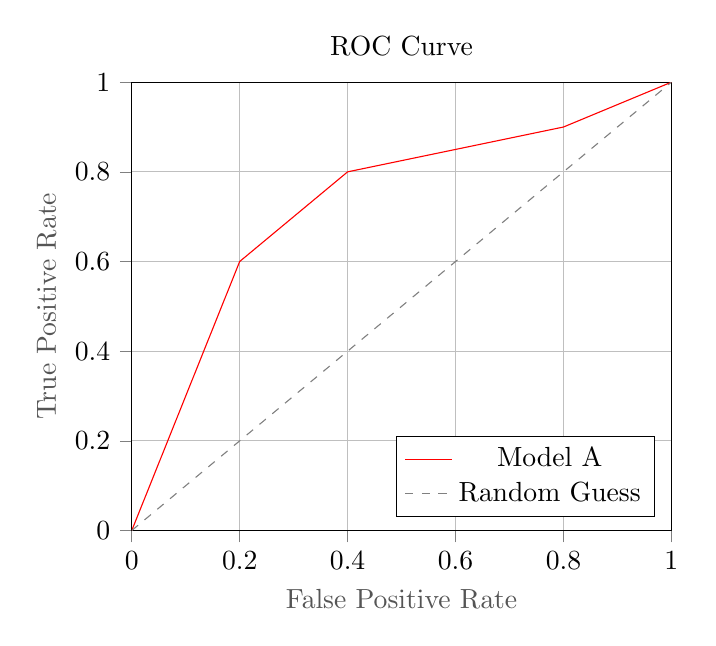
\begin{tikzpicture}
        \definecolor{darkorange}{RGB}{255,140,0}
        \definecolor{dimgray85}{RGB}{85,85,85}
        \definecolor{lightgray}{RGB}{211,211,211}
        \definecolor{lightgray204}{RGB}{204,204,204}
    \definecolor{navy}{RGB}{0,0,128}
        \begin{axis}[
            grid=major,
            xmin=0, xmax=1,
            ymin=0, ymax=1,
            title=ROC Curve,
            legend pos=south east,
            ylabel=\textcolor{dimgray85}{True Positive Rate},
            xlabel=\textcolor{dimgray85}{False Positive Rate},
            xtick={0, 0.2,0.4,0.6,0.8,1},
            ytick={0, 0.2,0.4,0.6,0.8,1},
            tick align=outside,
            tick pos=left,
        ]
            \addplot[color=red, mark=none] coordinates {
                (0,0)
                (0.1,0.3)
                (0.2,0.6)
                (0.3,0.7)
                (0.4,0.8)
                (0.6,0.85)
                (0.8,0.9)
                (1,1)
            };
            \addlegendentry{Model A}
            \addplot[dashed, gray] coordinates {(0,0) (1,1)};
            \addlegendentry{Random Guess}
        \end{axis}
    \end{tikzpicture}
    \caption{GPT 4 Receiver Operating Characteristic (ROC) Curve}
\end{figure}


\end{document}
